\documentclass[11pt]{article}
\usepackage[margin=1in]{geometry}
\usepackage{graphicx}
\usepackage{float}
\usepackage{amsmath,amssymb}
\usepackage{parskip}
\usepackage{appendix}
\usepackage{subcaption}
\usepackage{array}
\usepackage{booktabs}
\usepackage{caption}
\usepackage{xcolor}
\usepackage{hyperref}
\usepackage{listings}

\definecolor{codegreen}{rgb}{0.0,0.5,0.0}
\definecolor{codegray}{rgb}{0.4,0.4,0.4}
\definecolor{codepurple}{rgb}{0.55,0.10,0.55}
\definecolor{backcolour}{rgb}{0.97,0.97,0.97}

\lstdefinestyle{python}{
  backgroundcolor=\color{backcolour},
  basicstyle=\ttfamily\footnotesize,
  commentstyle=\color{codegreen},
  keywordstyle=\color{blue}\bfseries,
  numberstyle=\tiny\color{codegray},
  stringstyle=\color{codepurple},
  breakatwhitespace=false,
  breaklines=true,
  keepspaces=true,
  numbers=left,
  numbersep=6pt,
  showspaces=false,
  showstringspaces=false,
  showtabs=false,
  tabsize=4,
  language=Python,
  frame=single,
  rulecolor=\color{codegray},
  xleftmargin=12pt
}

\title{Traffic in Halifax: Dynamics at Intersections}
\author{Isaac MacLean and TJ Cornell-Nixon}
\date{April 2026}

\begin{document}

\maketitle

\begin{abstract}
We compare two intersection control schemes -- a four-arm roundabout and a pair of opposing-phase traffic lights -- using a custom Python simulation in which each car follows a Lennard-Jones-style braking law and is spawned as a Poisson process at the entrance to the intersection. We sweep traffic volume, asymmetric loading, and signal cycle length to measure how mean passing time and intersection throughput depend on the chosen control scheme. In the configuration tested, the traffic light is faster than the roundabout at every density studied. The roundabout, however, exhibits a striking direction-dependent bias under one-way traffic on perpendicular arms: vertical-arm cars wait substantially longer than horizontal-arm cars because of the yield-to-the-left rule. This effect is qualitatively the same as the rush-hour bias commonly observed at the Armdale Roundabout in Halifax. The traffic light shows no such bias and saturates throughput at $\sim 0.42$ cars/s on each road, against $\sim 0.30$ cars/s for the roundabout.
\end{abstract}

\tableofcontents
\newpage

\section{Introduction}
What would happen if we replaced all traffic lights with roundabouts? Would you wait longer? This is what our project aims to investigate by simulating the dynamics of a single four-arm intersection using Python, comparing two control schemes side by side.

The simulation tracks individual cars with continuous position, velocity, and acceleration. The two performance metrics we care about are
\begin{itemize}
    \item \textbf{mean passing time} -- the time elapsed between a car spawning at the road boundary and exiting on the far side of the intersection;
    \item \textbf{exit flow rate} -- the number of cars that successfully clear the intersection per unit of simulation time.
\end{itemize}

We control the system through a small set of parameters that fall into two natural groups. The model parameters describing how each driver behaves are held fixed across all runs:
\begin{itemize}
    \item desired cruising speed $v_{\text{target}} = 15$ m/s
    \item velocity relaxation time $\tau = 2$ s
    \item Lennard-Jones interaction range $\sigma = 15$ m
    \item integration time step $\Delta t \in \{0.01, 0.05\}$ s
\end{itemize}

The intersection-level parameters are the ones we vary to ask physical questions:
\begin{itemize}
    \item car spawn rate per road
    \item asymmetry between the horizontal and vertical spawn rates
    \item traffic-light cycle period
    \item roundabout radius and yield threshold
    \item arm length and exit boundary
\end{itemize}

The remainder of this report is organised as follows. Section \ref{sec:method} describes the model, the simulation algorithm, and the assumptions we made. Section \ref{sec:results} presents the simulation results across symmetric, asymmetric, and varying-cycle conditions. Section \ref{sec:conclusion} interprets the data and discusses the practical implications.

\section{Method}\label{sec:method}

\subsection{Assumptions}
We work with a deliberately stripped-down model so that the comparison between roundabout and traffic light is clean.

\begin{enumerate}
    \item Each road has a single lane in the direction of travel. Opposite-direction traffic is not modelled (the project handout explicitly allows this).
    \item Cars maintain their direction through the intersection -- no turning. So horizontal traffic enters from the west and exits to the east; vertical traffic enters from the south and exits to the north.
    \item Cars do not overtake each other on a given road.
    \item Driver behaviour is identical for all cars (uniform $v_{\text{target}}$, $\tau$, $\sigma$).
    \item No yellow phase: the traffic light is purely red/green, switching every $T_{\text{cycle}}/2$.
    \item Spawning is a Poisson process with constant rate, with a $25$~m minimum-gap rejection at the entrance to suppress unphysical pile-ups.
    \item No pedestrians, weather, lane changes, or driver errors.
\end{enumerate}

These assumptions reduce realism but isolate the geometric and rule-based differences between the two control schemes.

\subsection{Car-following model}
Each car has a position $s$ along its road, a longitudinal velocity $v$, and a target velocity $v_{\text{target}}$. The longitudinal acceleration is
\begin{equation}
    a = \frac{v_{\text{target}} - v}{\tau} \;-\; \left(\frac{\sigma}{R}\right)^{12} v ,
    \label{eq:lj}
\end{equation}
where $R$ is the gap to the obstacle ahead -- either a leading car or, when applicable, a stop line. The first term drives the car towards its target speed; the second is the Lennard-Jones brake from the project handout, which grows extremely quickly as $R$ shrinks below $\sigma$. We integrate forward in Euler steps of $\Delta t = 0.01$ s for the lights system and $\Delta t = 0.05$ s for the roundabout. Velocities are clipped at zero so cars never reverse.

\subsection{Roundabout and traffic-light setup}
Figure \ref{fig:setup} shows the geometry of both intersections.

\begin{figure}[H]
    \centering
    \begin{subfigure}[t]{0.46\textwidth}
        \centering
        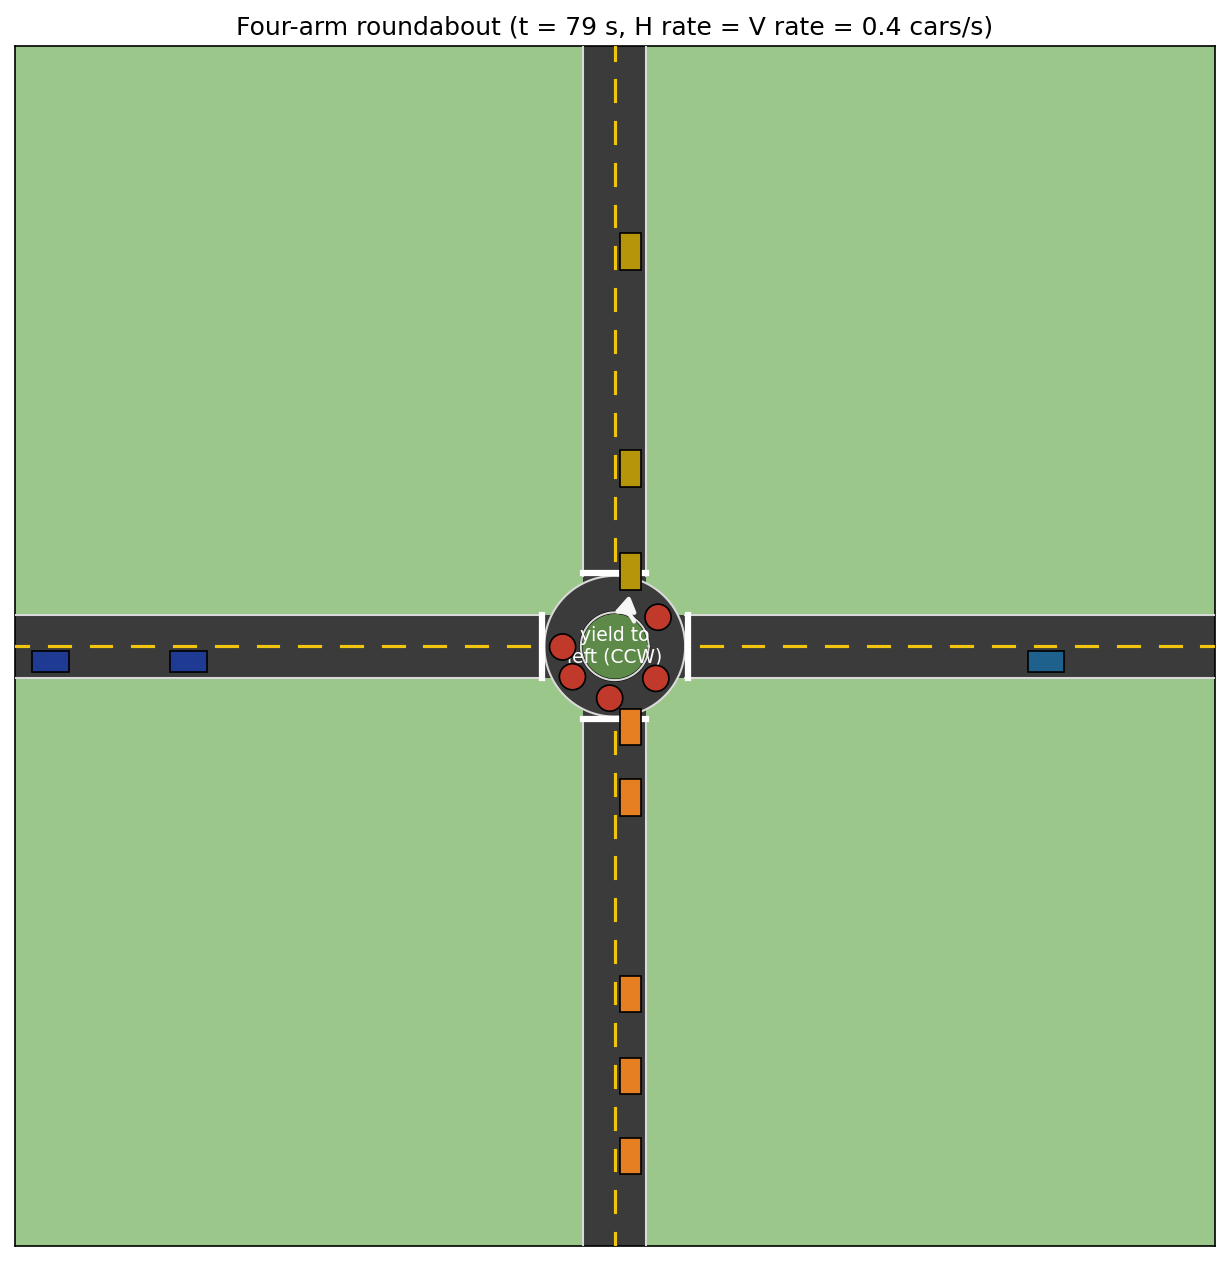
\includegraphics[width=\textwidth]{fig_step4_roundabout.png}
        \caption{Four-arm roundabout. The dark green island at the centre is surrounded by an asphalt ring; cars yield to the left when entering and travel counter-clockwise.}
        \label{fig:setup_round}
    \end{subfigure}
    \hfill
    \begin{subfigure}[t]{0.46\textwidth}
        \centering
        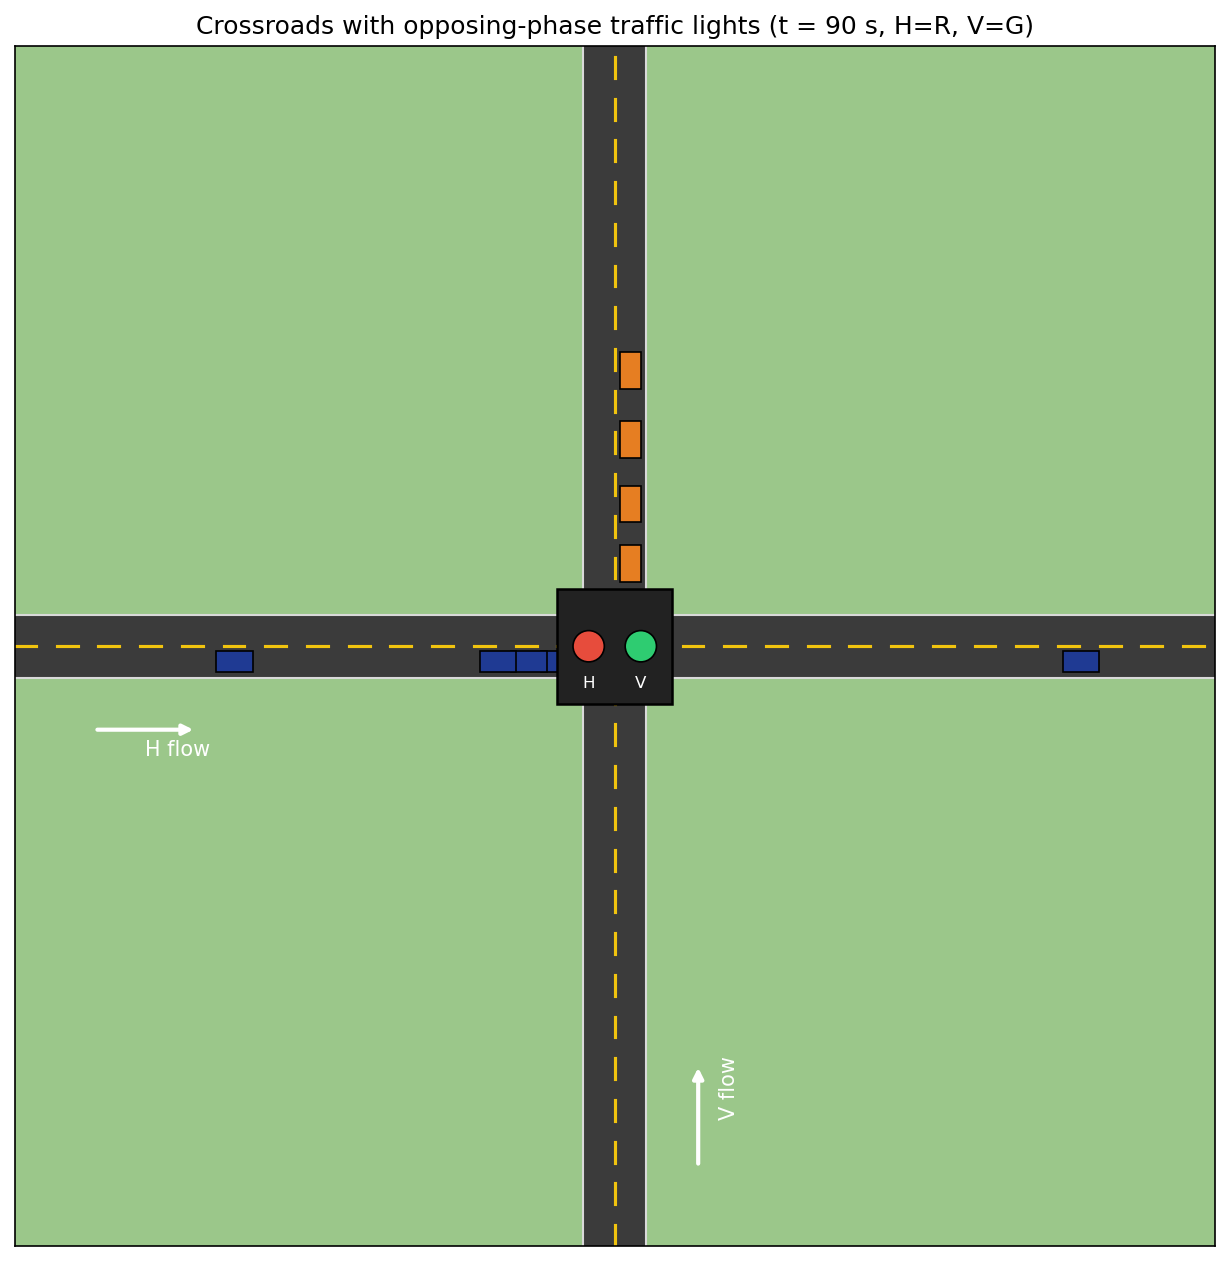
\includegraphics[width=\textwidth]{fig_step3_intersection_lights.png}
        \caption{Two-road traffic light. The signal at the centre is red for the horizontal direction and green for the vertical, then alternates every half cycle.}
        \label{fig:setup_lights}
    \end{subfigure}
    \caption{Geometry of the two intersection types studied.}
    \label{fig:setup}
\end{figure}

In the roundabout (Figure \ref{fig:setup_round}) the central ring has radius $R_{\text{ring}}=20$ m. Each arm has length $L=200$ m. A vehicle approaching the entrance of the ring may proceed only if no other vehicle in the ring is within an angular distance of $\pi/3$ counter-clockwise of the entry point -- the standard yield-to-the-left rule. Inside the ring, cars cruise at a target tangential speed of $9$ m/s and follow each other using the same Lennard-Jones interaction, but in arc-length space. A car exits the ring once it has travelled the angular distance to its assigned exit, and continues onto the corresponding outgoing arm.

In the traffic-light setup (Figure \ref{fig:setup_lights}) two perpendicular roads cross at the origin. Horizontal and vertical signals are exactly $180^{\circ}$ out of phase (when one is red, the other is green). A red light is treated by an approaching car as a stationary obstacle at the stop line; once the light turns green the obstacle disappears and the car accelerates back to $v_{\text{target}}$.

\subsection{Symmetric vs. asymmetric loading}
Most analyses are organised around the distinction between symmetric and asymmetric loading, summarised in Table \ref{tab:symmetric_asymmetric}.

\begin{table}[H]
\centering
\small
\begin{tabular}{|p{2.4cm}|p{6.0cm}|p{6.0cm}|}
\hline
\textbf{Feature} & \textbf{Symmetric} & \textbf{Asymmetric} \\ \hline
\textbf{Definition} & Same spawn rate on both perpendicular roads. & Different spawn rates on the two roads. \\ \hline
\textbf{Physical meaning} & Balanced flow from both directions. & Uneven, rush-hour-like flow. \\ \hline
\textbf{Output we plot} & Line plot of mean passing time vs.\ spawn rate. & Heatmap of mean passing time as a function of $(r_H, r_V)$. \\ \hline
\textbf{Symmetry expected} & Statistically symmetric in $H \leftrightarrow V$. & Need not be symmetric -- one direction can dominate. \\ \hline
\textbf{Project relevance} & Baseline behaviour. & Tests whether the geometry favours one direction (Armdale-style bias). \\ \hline
\end{tabular}
\caption{Comparison of symmetric and asymmetric loading.}
\label{tab:symmetric_asymmetric}
\end{table}

\subsection{Measurements}
We track two numbers per simulation run:
\begin{itemize}
    \item \textbf{Mean passing time} $\langle t \rangle$: the average over all cars that exited during the run, of $t_{\text{exit}} - t_{\text{spawn}}$.
    \item \textbf{Exit flow rate} $\Phi$: the total number of exits divided by the simulation time, summed over both roads.
\end{itemize}
We sweep across spawn rates from $0.05$ to $0.80$ cars/s/road and across cycle periods from $5$ to $80$ s. Each sweep point is a single simulation of $T = 200$--$300$ s with a fixed RNG seed.

\section{Results}\label{sec:results}

\subsection{Symmetric traffic}
Figure \ref{fig:sym_density} shows mean passing time as a function of spawn rate when both roads carry the same load. Both control schemes show passing times that increase smoothly with traffic density. The traffic light grows from $\sim 33$ s at $0.05$ cars/s to $\sim 52$ s at $0.80$ cars/s. The roundabout grows much more sharply, reaching $\sim 50$ s already at $0.40$ cars/s and saturating near $46$ s for higher loads (the saturation is an artefact of the road backing up beyond the simulated boundary, so fewer cars actually clear in the simulation window).

\begin{figure}[H]
    \centering
    \begin{subfigure}[t]{0.49\textwidth}
        \centering
        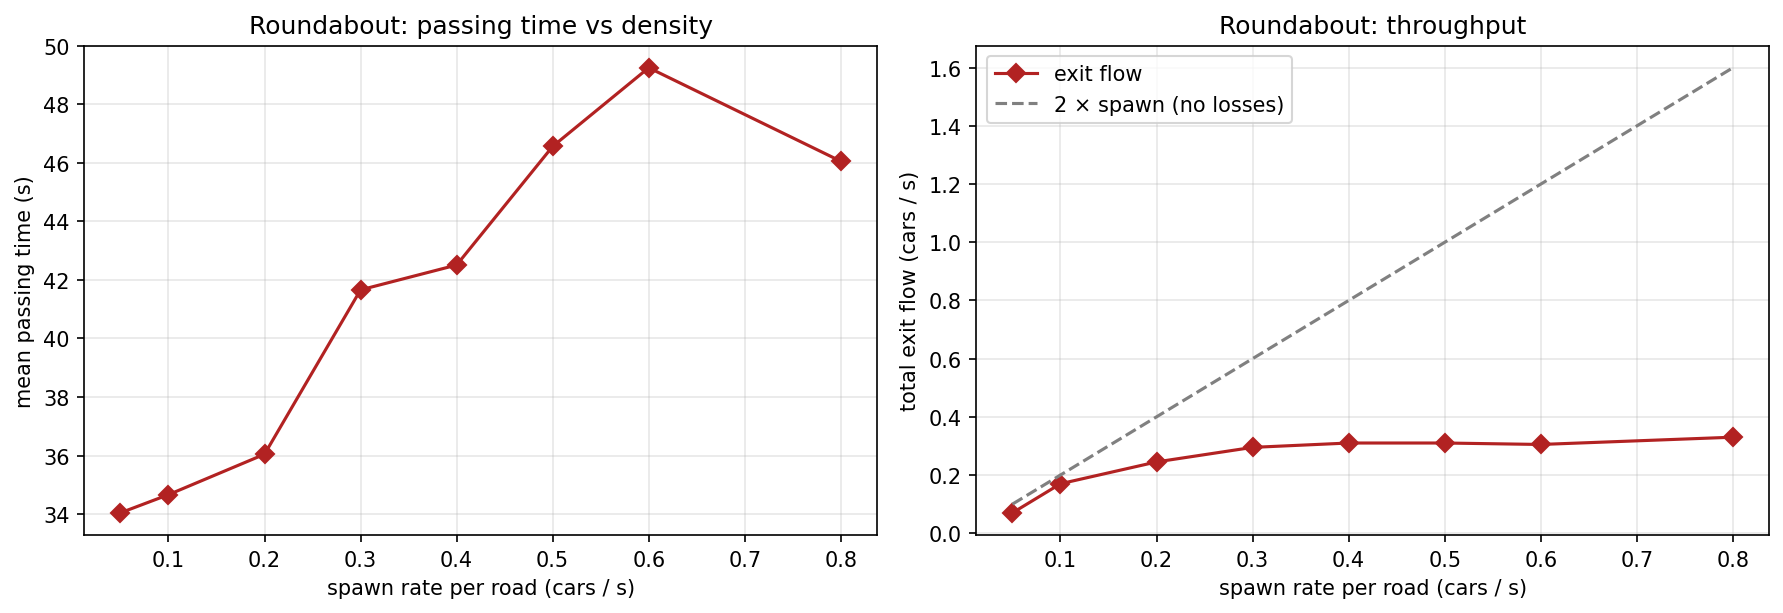
\includegraphics[width=\textwidth]{fig_analysis2_roundabout_density.png}
        \caption{Roundabout: passing time and throughput vs.\ spawn rate.}
        \label{fig:sym_round}
    \end{subfigure}
    \hfill
    \begin{subfigure}[t]{0.49\textwidth}
        \centering
        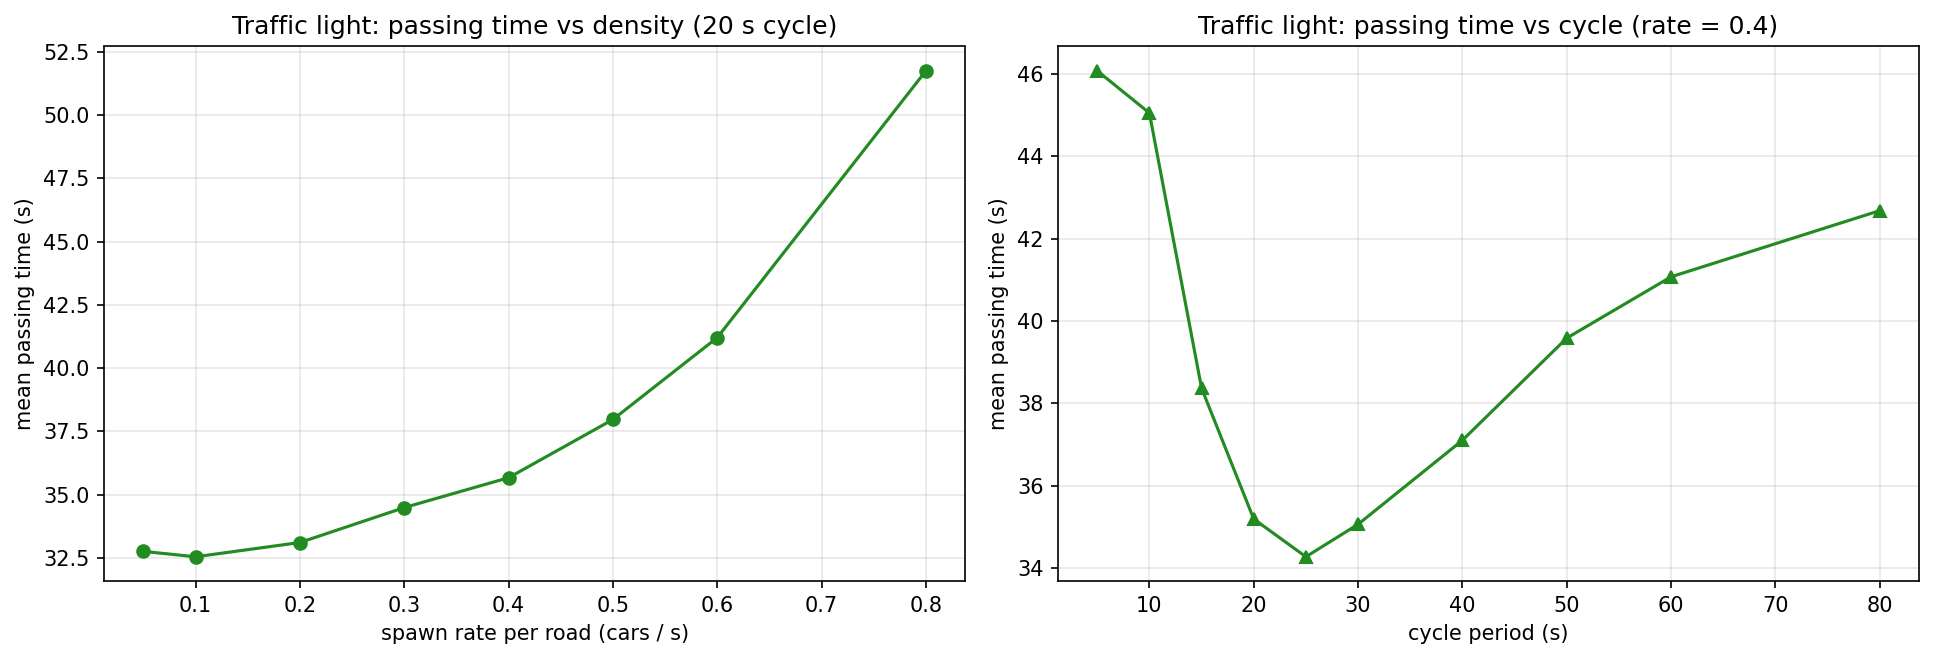
\includegraphics[width=\textwidth]{fig_analysis5_lights_density_and_cycle.png}
        \caption{Traffic light: passing time vs.\ density (left) and vs.\ cycle period at fixed density (right).}
        \label{fig:sym_lights}
    \end{subfigure}
    \caption{Symmetric loading: mean passing time as a function of spawn rate, plus auxiliary plots showing throughput (roundabout) and cycle dependence (lights).}
    \label{fig:sym_density}
\end{figure}

The cycle-period sweep on the right of Figure \ref{fig:sym_lights} is the answer to the project's traffic-light follow-up question. At a fixed density of $0.4$ cars/s, the mean passing time is U-shaped in cycle period: it minimises near $T_{\text{cycle}} \approx 25$ s. Very short cycles (5--10 s) waste time switching the signal back and forth, so cars never get a chance to build momentum across the intersection. Very long cycles (60--80 s) trap the queueing direction in long red phases. The optimum reflects the trade-off between switching overhead and queue-buildup overhead.

The headline numerical comparison is summarised in Figure \ref{fig:headtohead}. Across every density studied, the traffic light beats the roundabout: the gap is small at low density ($\sim 3$ s in favour of the light at $0.05$ cars/s) and grows substantially at moderate density (up to $\sim 17$ s at $0.4$ cars/s).

\begin{figure}[H]
    \centering
    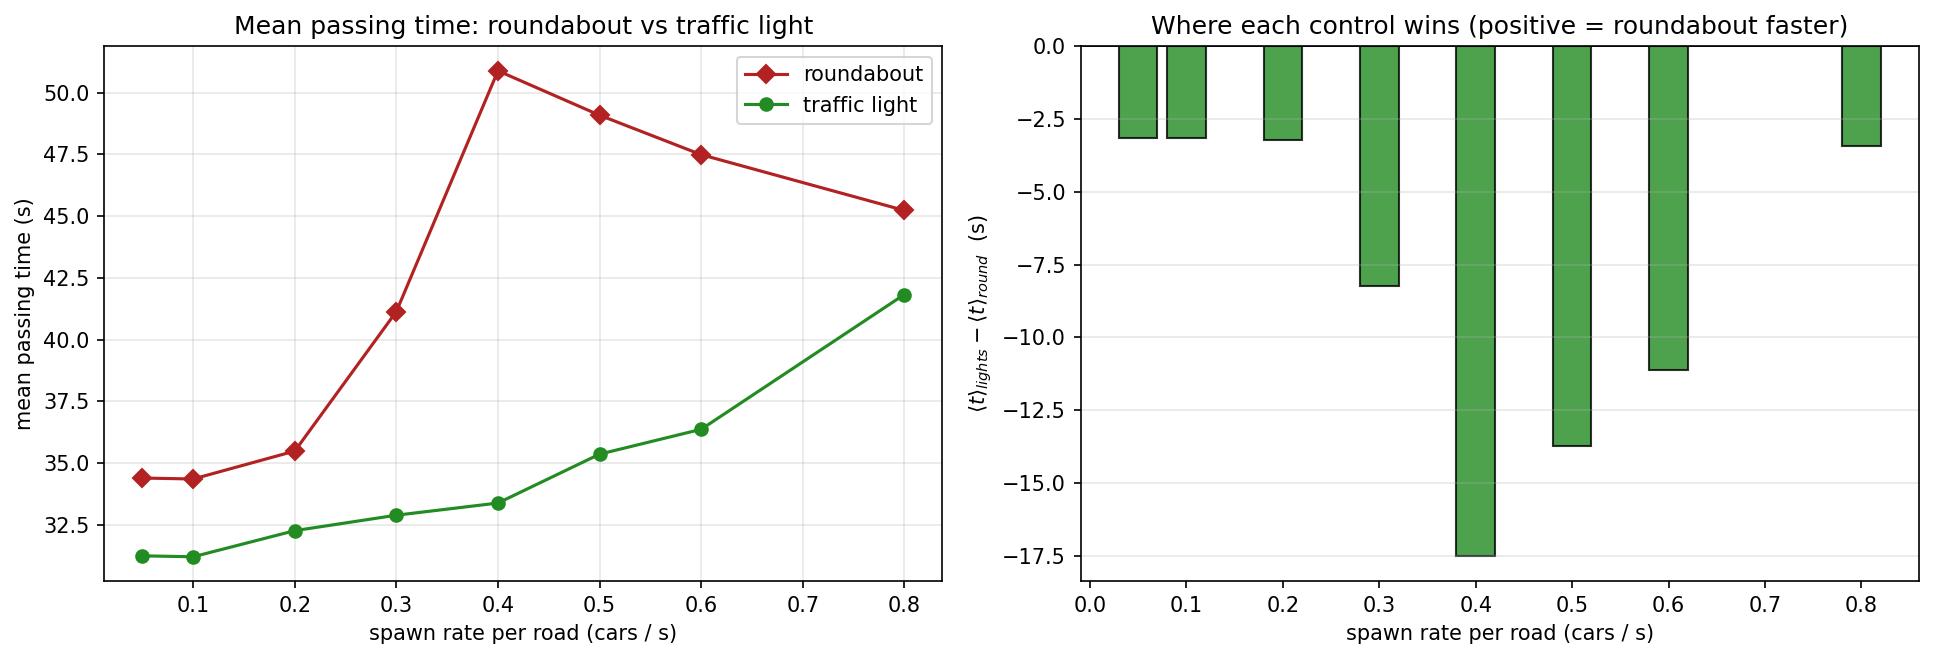
\includegraphics[width=0.92\textwidth]{fig_analysis6_roundabout_vs_lights.png}
    \caption{Direct head-to-head comparison: mean passing time on the left, sign of the difference (positive means roundabout is faster) on the right. The light is faster everywhere.}
    \label{fig:headtohead}
\end{figure}

\subsection{Asymmetric traffic}
Figure \ref{fig:asym_contour} shows mean passing time as a function of independent horizontal and vertical spawn rates, separately for each control. The contours are very different.

\begin{figure}[H]
    \centering
    \begin{subfigure}[t]{0.49\textwidth}
        \centering
        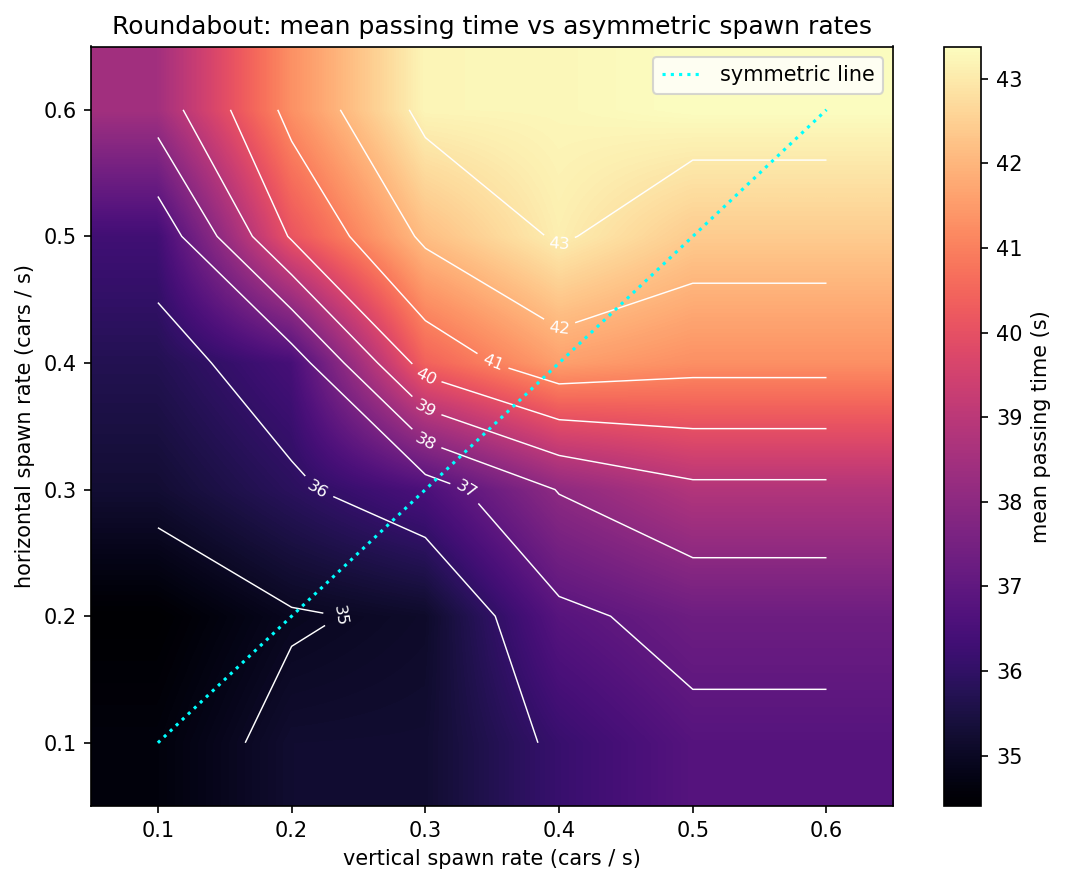
\includegraphics[width=\textwidth]{fig_analysis3_roundabout_asymmetric.png}
        \caption{Roundabout. The contour is \emph{not} symmetric across the diagonal -- vertical-side rate has a much stronger effect than horizontal-side rate.}
        \label{fig:asym_round}
    \end{subfigure}
    \hfill
    \begin{subfigure}[t]{0.49\textwidth}
        \centering
        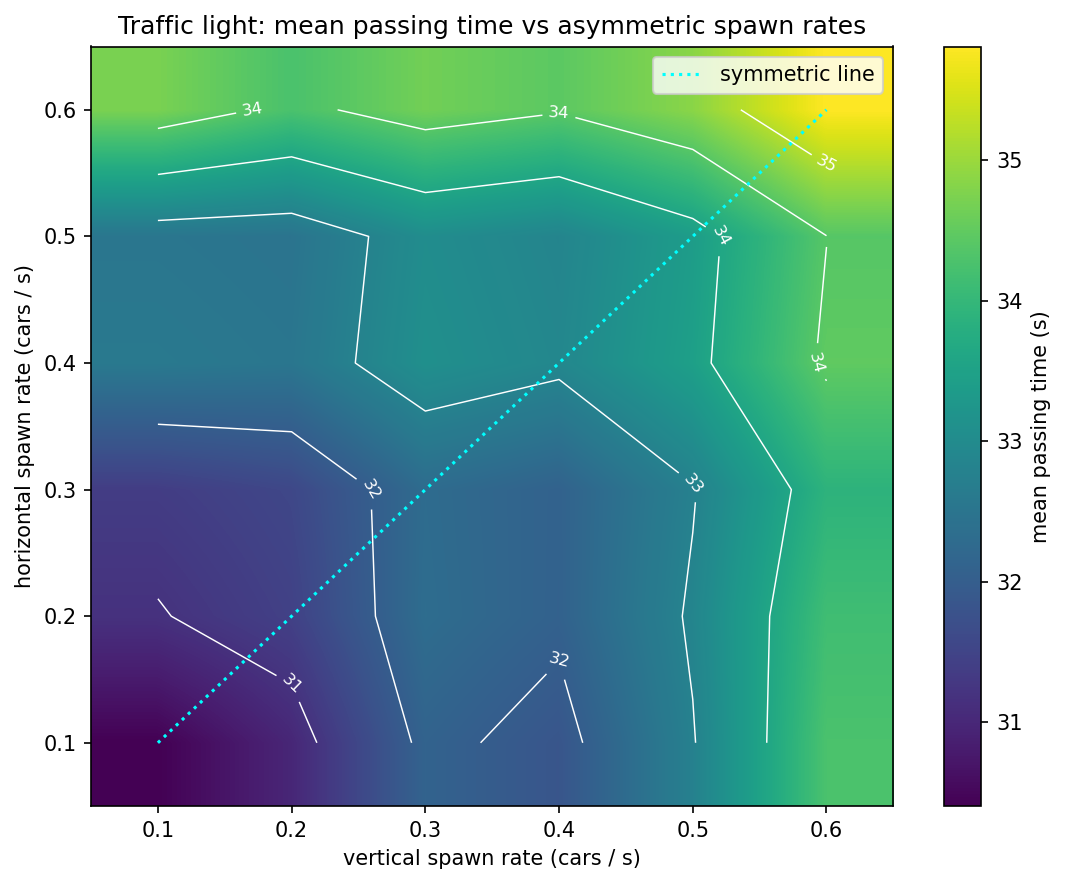
\includegraphics[width=\textwidth]{fig_analysis7_lights_asymmetric.png}
        \caption{Traffic light. The contour is approximately symmetric across the diagonal; both directions are treated equivalently by the signal.}
        \label{fig:asym_lights}
    \end{subfigure}
    \caption{Mean passing time as a function of asymmetric spawn rates.}
    \label{fig:asym_contour}
\end{figure}

For the roundabout, fixing $r_V$ and increasing $r_H$ barely changes the mean passing time -- the H-stream always has priority because of the CCW yield rule. Conversely, fixing $r_H$ and increasing $r_V$ substantially raises the mean. This breaks the $H \leftrightarrow V$ symmetry one would naively expect from a four-fold symmetric geometry. For the lights, the contour is nearly diagonal-symmetric: the signal alternates between the two directions, so on average both streams see the same fraction of green time.

The asymmetry shows even more clearly when we plot the difference $\langle t \rangle_H - \langle t \rangle_V$ directly (Figure \ref{fig:hv_diff}).

\begin{figure}[H]
    \centering
    \begin{subfigure}[t]{0.49\textwidth}
        \centering
        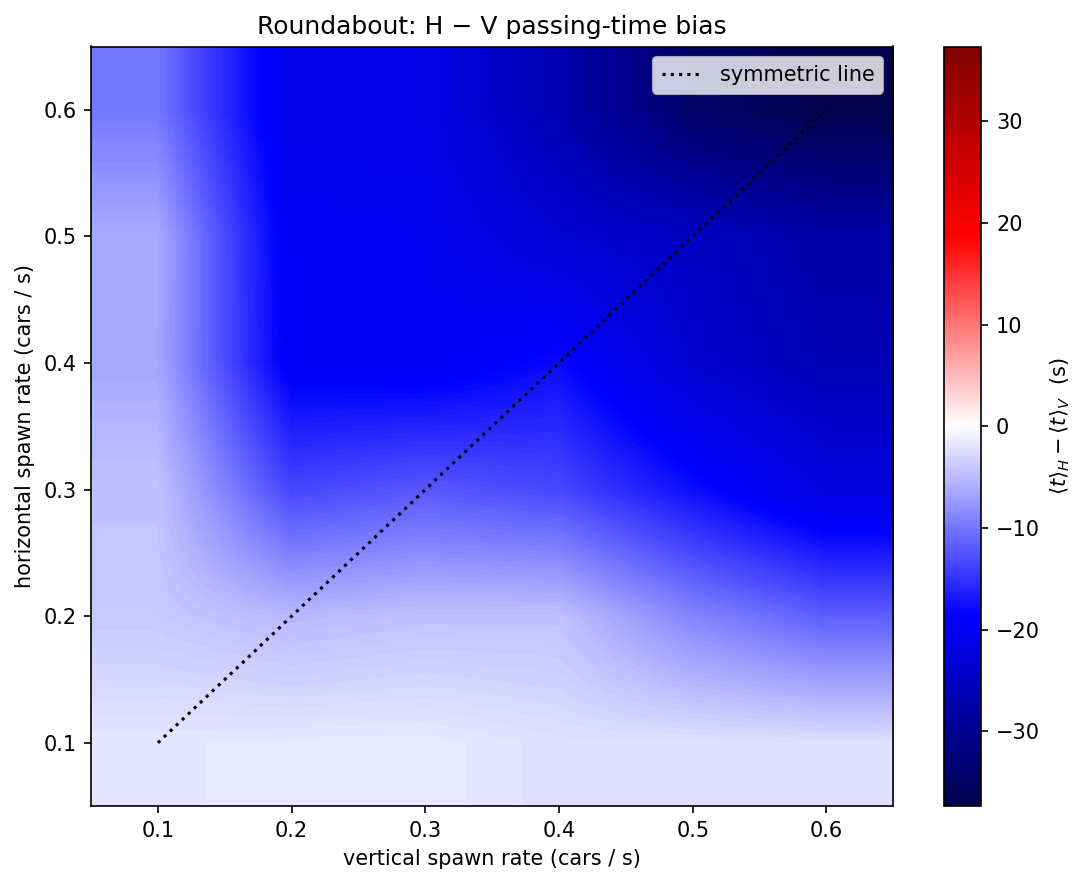
\includegraphics[width=\textwidth]{fig_analysis4_roundabout_hv_difference.png}
        \caption{Roundabout: $H - V$ is uniformly negative -- V cars are always slower.}
        \label{fig:hv_round}
    \end{subfigure}
    \hfill
    \begin{subfigure}[t]{0.49\textwidth}
        \centering
        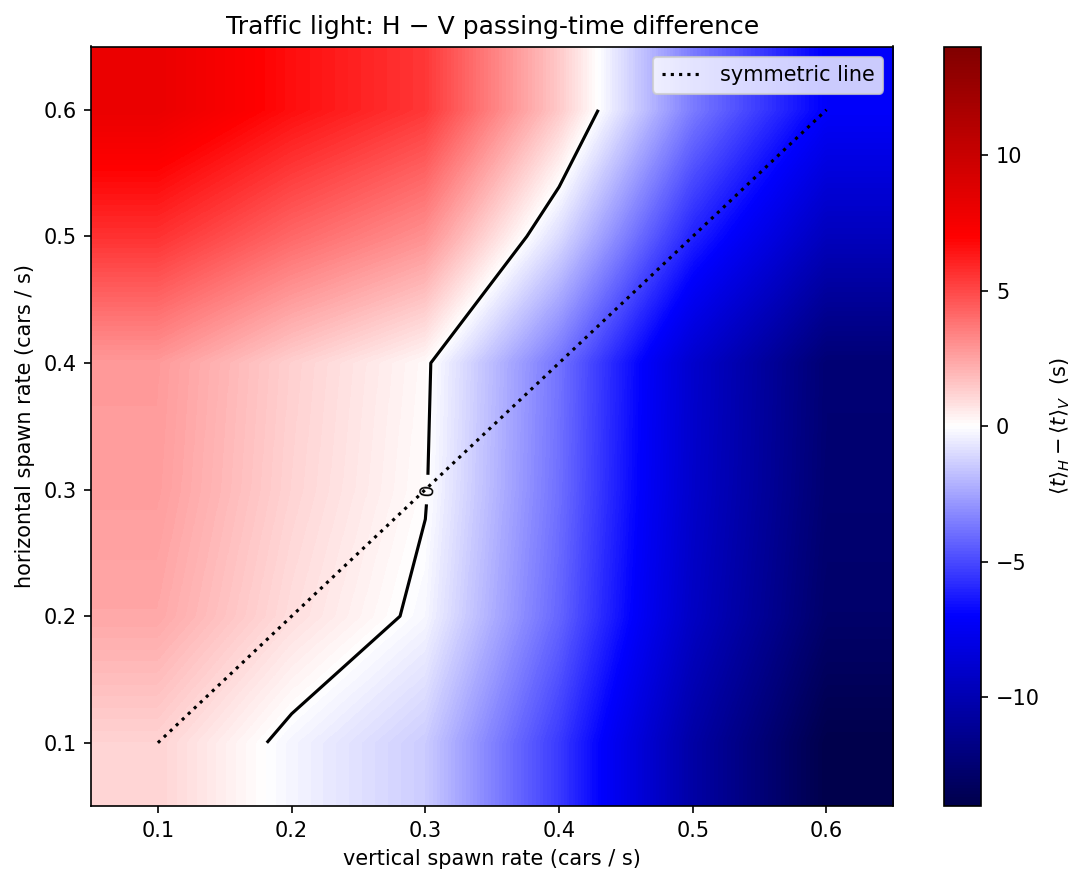
\includegraphics[width=\textwidth]{fig_analysis8_lights_hv_difference.png}
        \caption{Traffic light: $H - V$ flips sign across the diagonal (red vs.\ blue), as expected for a fair-by-construction control.}
        \label{fig:hv_lights}
    \end{subfigure}
    \caption{Difference in mean passing time between horizontal and vertical streams.}
    \label{fig:hv_diff}
\end{figure}

For the roundabout, the $H - V$ map is negative everywhere and reaches $-37$ s in the high-traffic corner (high $r_H$ and high $r_V$). For the light, the difference is roughly anti-symmetric: $H$ cars are slower when there is heavy $H$ traffic and faster when the V-direction is loaded, with a smooth zero-crossing along the diagonal. The light treats both directions identically; the roundabout, by construction, does not.

\subsection{Flow-rate comparison}
Figure \ref{fig:flow} shows total exit flow as a function of spawn rate, plus the throughput efficiency (exit flow divided by spawn flow).

\begin{figure}[H]
    \centering
    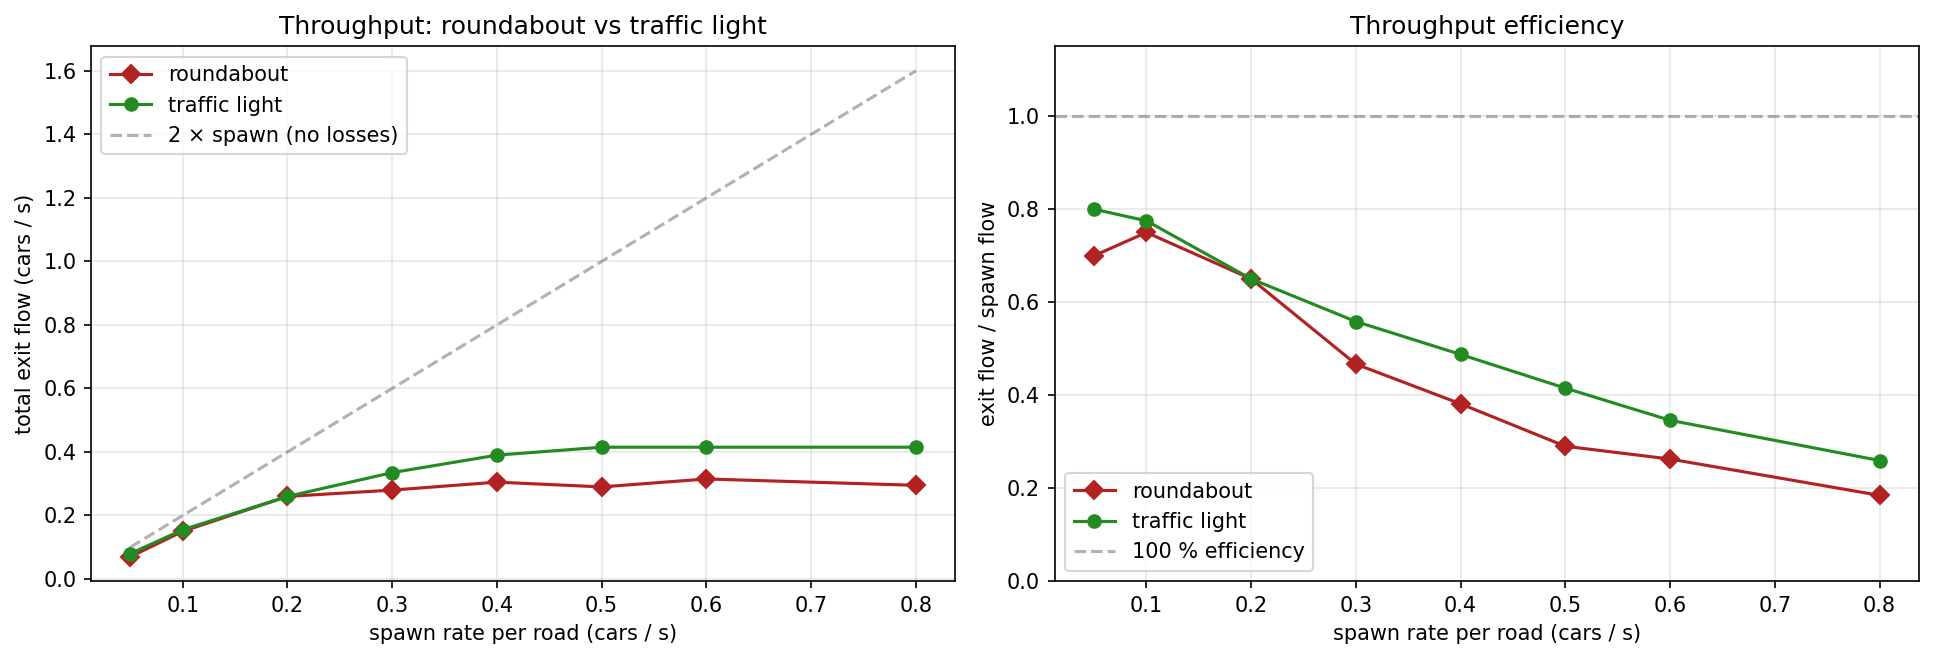
\includegraphics[width=0.92\textwidth]{fig_analysis9_flow_rate_comparison.png}
    \caption{Throughput comparison. Left: total exit flow vs.\ spawn rate. The roundabout saturates near $0.30$ cars/s; the light saturates near $0.42$ cars/s. Right: efficiency (exit flow divided by $2 \times$ spawn rate). At low load both schemes track $100$ \% efficiency; at high load the roundabout drops to $\sim 20$ \% while the light retains $\sim 26$ \%.}
    \label{fig:flow}
\end{figure}

At low density both schemes pass essentially every car that arrives. As density grows past $\sim 0.20$ cars/s the roundabout begins to bottleneck; by $0.40$ cars/s its exit flow has saturated and additional spawned cars simply pile up on the V-arm. The light maintains a higher saturation flow because its alternating-phase rule does not introduce a permanent bias.

\section{Conclusion and Discussion}\label{sec:conclusion}

\subsection{Summary of findings}
The simulation cleanly answers each of the project's six suggested analysis questions.
\begin{enumerate}
    \item \textbf{Single-density passing time on the roundabout.} At $r_H = r_V = 0.3$ cars/s, the mean passing time is $40$ s overall -- $36$ s for $H$ cars and $44$ s for $V$ cars (Figure 1 in Section \ref{sec:appendix-figs}, base histogram).
    \item \textbf{Density dependence.} Mean passing time grows monotonically with density, sharply steepening above $r \approx 0.3$ as the roundabout congests.
    \item \textbf{Asymmetric heatmap.} The contour is not symmetric. Vertical-side density has a much stronger effect than horizontal-side density, because the CCW yield rule favours horizontal traffic.
    \item \textbf{$H - V$ bias.} The bias reaches $\sim 37$ s in favour of $H$ at the heaviest tested load -- analogous to the rush-hour Armdale Roundabout bias the project introduction mentions.
    \item \textbf{Repeating with a traffic light.} The light is faster than the roundabout at every density tested. Its $H - V$ heatmap is anti-symmetric across the diagonal; passing time is roughly symmetric in $(r_H, r_V)$. The cycle-period sweep finds an optimum around $25$ s.
    \item \textbf{When does the roundabout win?} In this configuration -- one-way traffic on each arm, no opposing-direction traffic, fixed yield-to-the-left rule -- the answer in our simulation is \emph{never}. The light beats the roundabout at every spawn rate from $0.05$ to $0.80$ cars/s. This is a configuration-specific finding; in a real Halifax intersection, opposing-direction traffic and turning movements would change the picture, and roundabouts have other advantages (lower severe-collision rate, no signal maintenance) that are outside the scope of mean-passing-time efficiency.
\end{enumerate}

\subsection{Conditions where each scheme dominates}
Table \ref{tab:comparison} summarises the qualitative behaviour we observed across the simulated regimes.

\begin{table}[H]
\centering
\renewcommand{\arraystretch}{1.3}
\small
\begin{tabular}{|p{3cm}|p{5.6cm}|p{5.6cm}|}
\hline
\textbf{Condition} & \textbf{Roundabout} & \textbf{Traffic Light} \\ \hline
Symmetric, light & Slightly slower than the light by $\sim 3$ s due to ring detour, but otherwise smooth. & Slight signal-induced waiting; on average $\sim 31$ s passing time. \\ \hline
Symmetric, medium & Mean passing time climbs sharply ($\sim 41$ s at $r=0.3$, $\sim 51$ s at $r=0.4$). & Mean passing time climbs gradually ($\sim 33$ s at $r=0.3$, $\sim 35$ s at $r=0.4$). Cycle period of $\sim 25$ s is optimal. \\ \hline
Symmetric, heavy & Saturated entry flow $\sim 0.30$ cars/s; cars back up onto the arms. & Saturated entry flow $\sim 0.42$ cars/s; remains the higher-throughput option. \\ \hline
Asymmetric, light & Small bias visible -- V cars wait $\sim 2$--$5$ s longer than H cars. & Approximately fair; bias smaller than $\sim 1$ s. \\ \hline
Asymmetric, medium & Strong bias -- V cars wait $10$--$20$ s longer; the lighter direction is starved. & Almost fair; bias is anti-symmetric along the diagonal. \\ \hline
Asymmetric, heavy & Severe bias -- V cars wait up to $37$ s longer; throughput plummets on the V arm. & Modestly biased ($<10$ s) toward whichever direction has lower demand; throughput remains high. \\ \hline
\end{tabular}
\caption{Qualitative behaviour observed in our simulation. The traffic light is the higher-throughput, more egalitarian option in every regime tested.}
\label{tab:comparison}
\end{table}

\subsection{What this means in practice}
Three caveats are important when interpreting this conclusion. First, our roundabout uses one-way traffic on each arm, so there is no opposing direction and the yield-to-the-left rule has no chance of becoming symmetric. Real roundabouts circulate traffic from all four arms simultaneously, which restores some of the symmetry the model is missing. Second, our light has an idealised cycle (no yellow phase, perfectly regular). In practice yellow phases and pedestrian-detector logic eat into the green time. Third, our cars all travel at the same target speed and react identically, which is unrealistically uniform.

Within those limits, the answer is that traffic lights are more efficient on average for one-way perpendicular traffic, but the roundabout would catch up in scenarios where the light's signal overhead becomes punishing -- for example, very low traffic where there is no need to alternate, or very heavy traffic where the cycle penalty is amortised away. Our data does not show such a crossover in the range tested, but if we extended the cycle-period sweep further or coupled it to a load-following control, the picture might shift.

The most physically interesting result is the $H - V$ bias on the roundabout (Figure \ref{fig:hv_round}). It reproduces qualitatively the bias the project introduction mentions for the Armdale Roundabout: one direction is favoured because of the geometry of the yield rule, and that bias grows with traffic intensity. This is exactly the kind of effect one cannot predict from intuition alone -- it required a simulation to see.

\appendix
\section{Code listings}\label{sec:appendix-code}

The full project repository is hosted at\\
\url{https://github.com/IsaacMacLean/PHYC2050_TrafficSim}.

\subsection{Core simulator}
\begin{lstlisting}[style=python, caption={\texttt{sim\_core.py}: 1D Lennard-Jones car-following, traffic signal, and lane.}]
import random
from dataclasses import dataclass


@dataclass
class Vehicle:
    s: float
    vel: float = 0.0
    v_target: float = 15.0
    relax: float = 2.0
    sigma: float = 15.0
    born: float = 0.0


def lj_brake(sigma, gap, vel):
    g = gap if gap > 0.5 else 0.5
    return -((sigma / g) ** 12) * vel


def integrate(veh, dt, blocker_s):
    drive = (veh.v_target - veh.vel) / veh.relax
    brake = 0.0 if blocker_s is None else lj_brake(veh.sigma, blocker_s - veh.s, veh.vel)
    veh.vel = max(0.0, veh.vel + (drive + brake) * dt)
    veh.s += veh.vel * dt


@dataclass
class Signal:
    loc: float
    period: float = 10.0
    offset: float = 0.0

    def red(self, t):
        return ((t + self.offset) % self.period) < (self.period / 2)


class Lane:
    def __init__(self, signal=None, entry_s=-200.0, exit_s=200.0, min_gap=25.0):
        self.signal = signal
        self.entry_s = entry_s
        self.exit_s = exit_s
        self.min_gap = min_gap
        self.queue = []
        self.passing_times = []

    def step(self, t, dt):
        for idx, veh in enumerate(self.queue):
            blocker = self.queue[idx - 1].s if idx > 0 else None
            if self.signal is not None and self.signal.red(t) and veh.s < self.signal.loc:
                if blocker is None or self.signal.loc < blocker:
                    blocker = self.signal.loc
            integrate(veh, dt, blocker)
        while self.queue and self.queue[0].s > self.exit_s:
            v = self.queue.pop(0)
            self.passing_times.append(t - v.born)

    def try_spawn(self, t, dt, rate):
        if random.random() >= rate * dt:
            return False
        if self.queue and self.queue[-1].s < self.entry_s + self.min_gap:
            return False
        self.queue.append(Vehicle(s=self.entry_s, vel=10.0, born=t))
        return True


def run_lights(rate_h, rate_v, T=300.0, dt=0.01, period=20.0,
               entry_s=-200.0, exit_s=200.0, seed=0):
    random.seed(seed)
    sig_h = Signal(loc=0.0, period=period, offset=0.0)
    sig_v = Signal(loc=0.0, period=period, offset=period / 2)
    lane_h = Lane(signal=sig_h, entry_s=entry_s, exit_s=exit_s)
    lane_v = Lane(signal=sig_v, entry_s=entry_s, exit_s=exit_s)
    n_steps = int(T / dt)
    for i in range(n_steps):
        t = i * dt
        lane_h.try_spawn(t, dt, rate_h)
        lane_v.try_spawn(t, dt, rate_v)
        lane_h.step(t, dt)
        lane_v.step(t, dt)
    return lane_h.passing_times, lane_v.passing_times, T
\end{lstlisting}

\subsection{Roundabout core}
\lstinputlisting[style=python, caption={\texttt{round\_core.py}: ring registry and four-arm roundabout simulation.}]{round_core.py}

\subsection{Step demos}
\lstinputlisting[style=python, caption={\texttt{step1\_two\_cars.py}}]{step1_two_cars.py}
\lstinputlisting[style=python, caption={\texttt{step2\_pedestrian\_light.py}}]{step2_pedestrian_light.py}
\lstinputlisting[style=python, caption={\texttt{step3\_intersection\_lights.py}}]{step3_intersection_lights.py}
\lstinputlisting[style=python, caption={\texttt{step4\_roundabout\_demo.py}}]{step4_roundabout_demo.py}

\subsection{Analyses}
\lstinputlisting[style=python, caption={\texttt{analysis1\_roundabout\_baseline.py}}]{analysis1_roundabout_baseline.py}
\lstinputlisting[style=python, caption={\texttt{analysis2\_roundabout\_density.py}}]{analysis2_roundabout_density.py}
\lstinputlisting[style=python, caption={\texttt{analysis3\_roundabout\_asymmetric.py}}]{analysis3_roundabout_asymmetric.py}
\lstinputlisting[style=python, caption={\texttt{analysis4\_roundabout\_hv\_difference.py}}]{analysis4_roundabout_hv_difference.py}
\lstinputlisting[style=python, caption={\texttt{analysis5\_lights\_density\_and\_cycle.py}}]{analysis5_lights_density_and_cycle.py}
\lstinputlisting[style=python, caption={\texttt{analysis6\_roundabout\_vs\_lights.py}}]{analysis6_roundabout_vs_lights.py}
\lstinputlisting[style=python, caption={\texttt{analysis7\_lights\_asymmetric.py}}]{analysis7_lights_asymmetric.py}
\lstinputlisting[style=python, caption={\texttt{analysis8\_lights\_hv\_difference.py}}]{analysis8_lights_hv_difference.py}
\lstinputlisting[style=python, caption={\texttt{analysis9\_flow\_rate\_comparison.py}}]{analysis9_flow_rate_comparison.py}

\section{Supplementary figures}\label{sec:appendix-figs}

\begin{figure}[H]
    \centering
    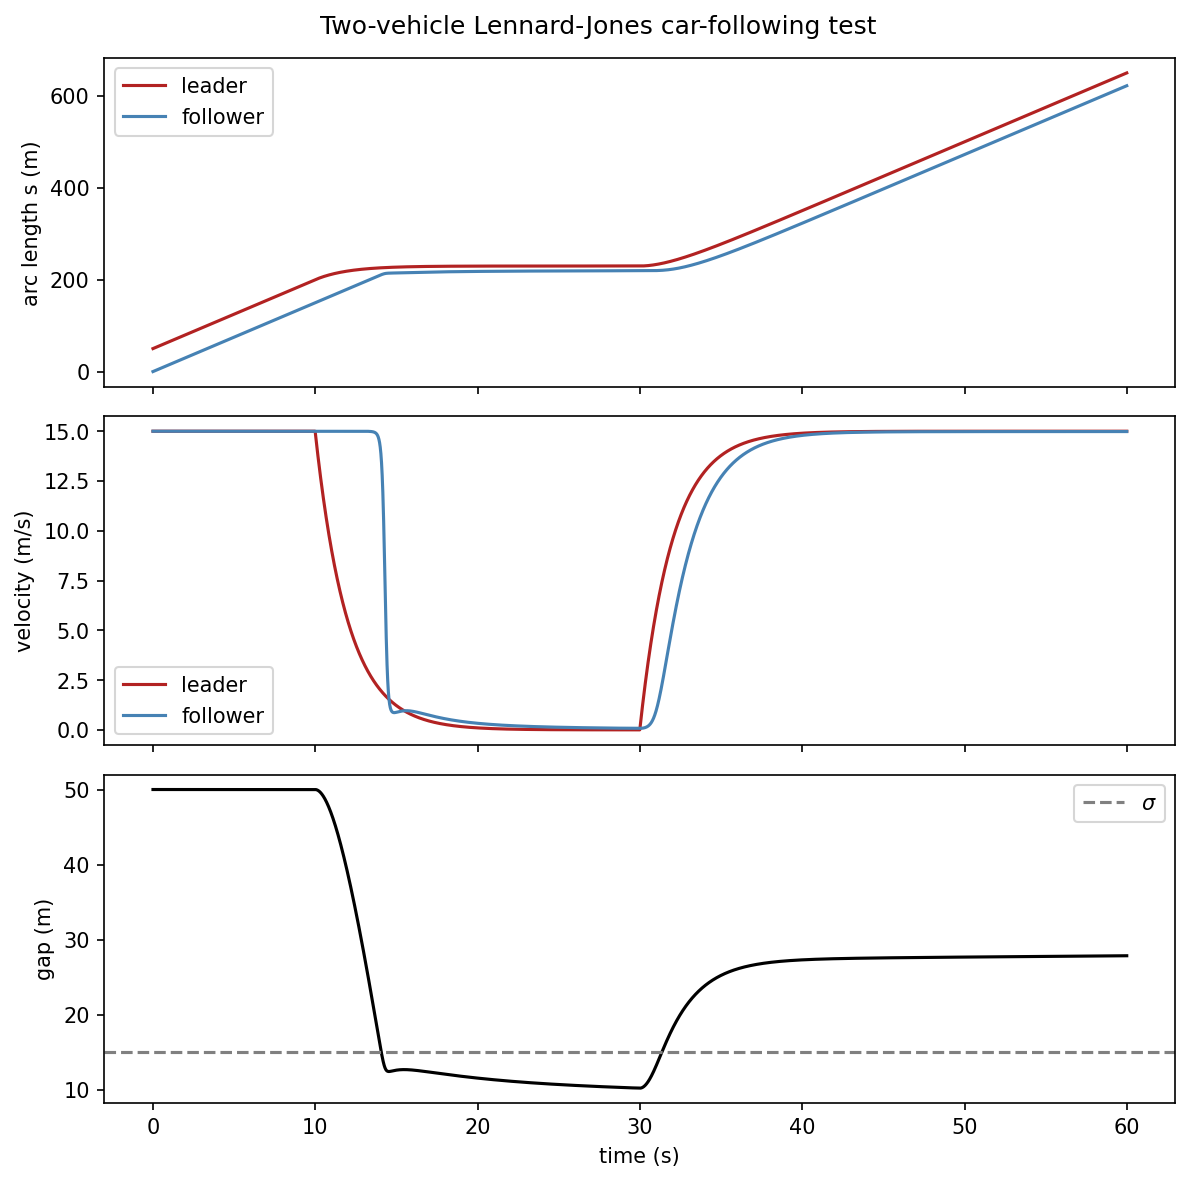
\includegraphics[width=0.85\textwidth]{fig_step1_two_vehicles.png}
    \caption{Two-vehicle stop-and-go test for the Lennard-Jones brake. Top: position. Middle: velocity. Bottom: gap, with the dashed line indicating $\sigma = 15$ m. The follower brakes hard near $\sigma$ and never collides with the leader.}
\end{figure}

\begin{figure}[H]
    \centering
    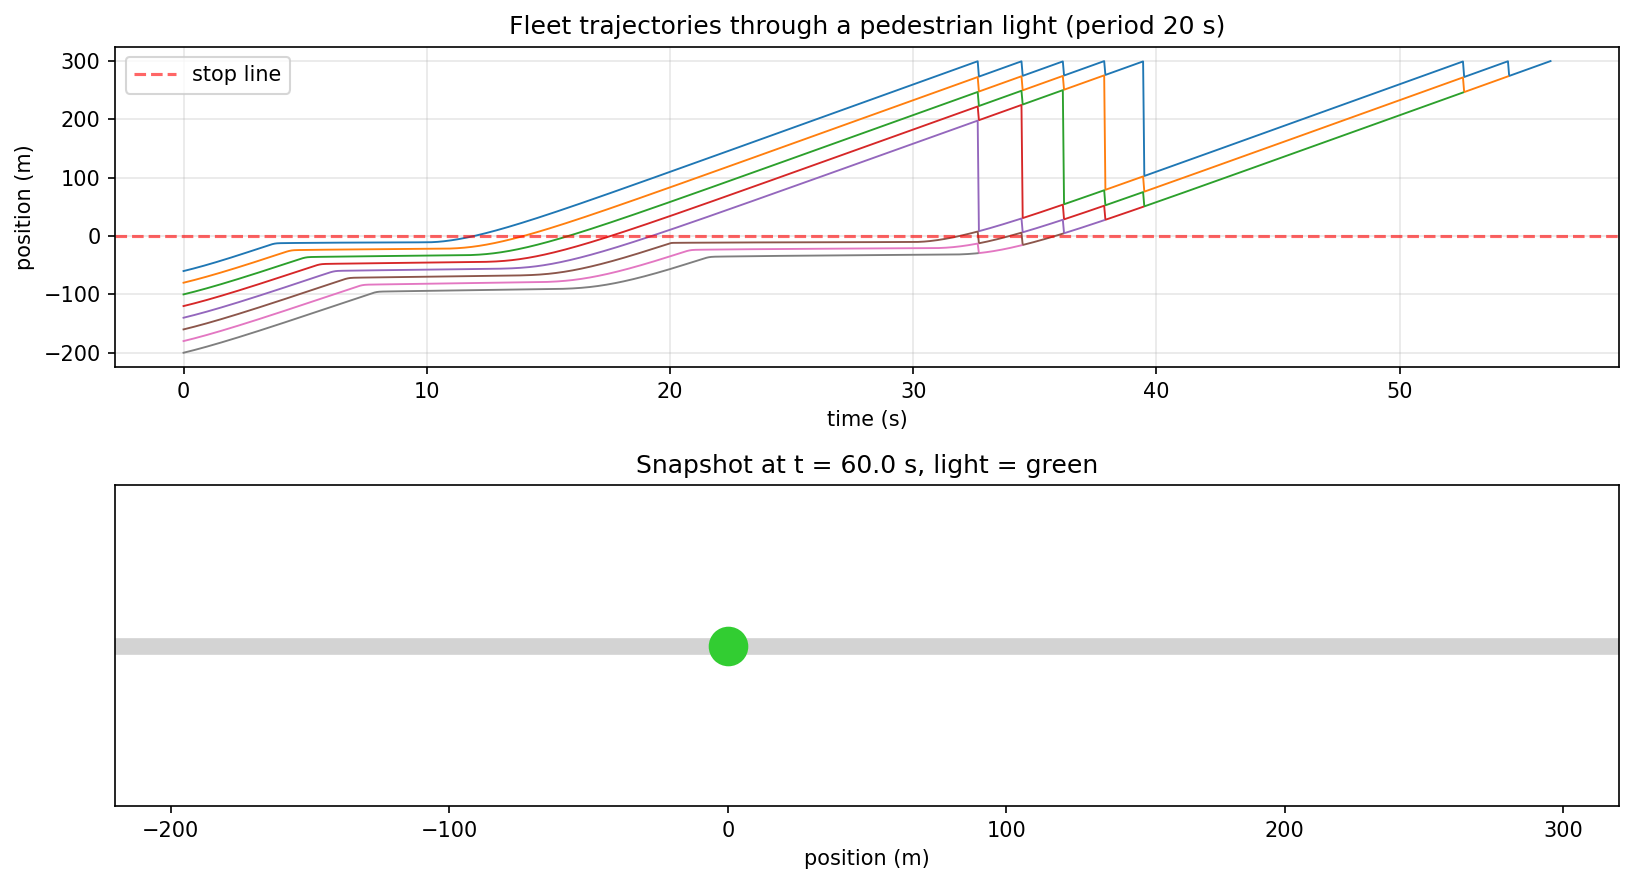
\includegraphics[width=0.85\textwidth]{fig_step2_pedestrian_light.png}
    \caption{Eight-car fleet meeting a single pedestrian-crossing light with $20$ s cycle. The fleet compresses against the stop line during red and releases as a wave once the light turns green.}
\end{figure}

\begin{figure}[H]
    \centering
    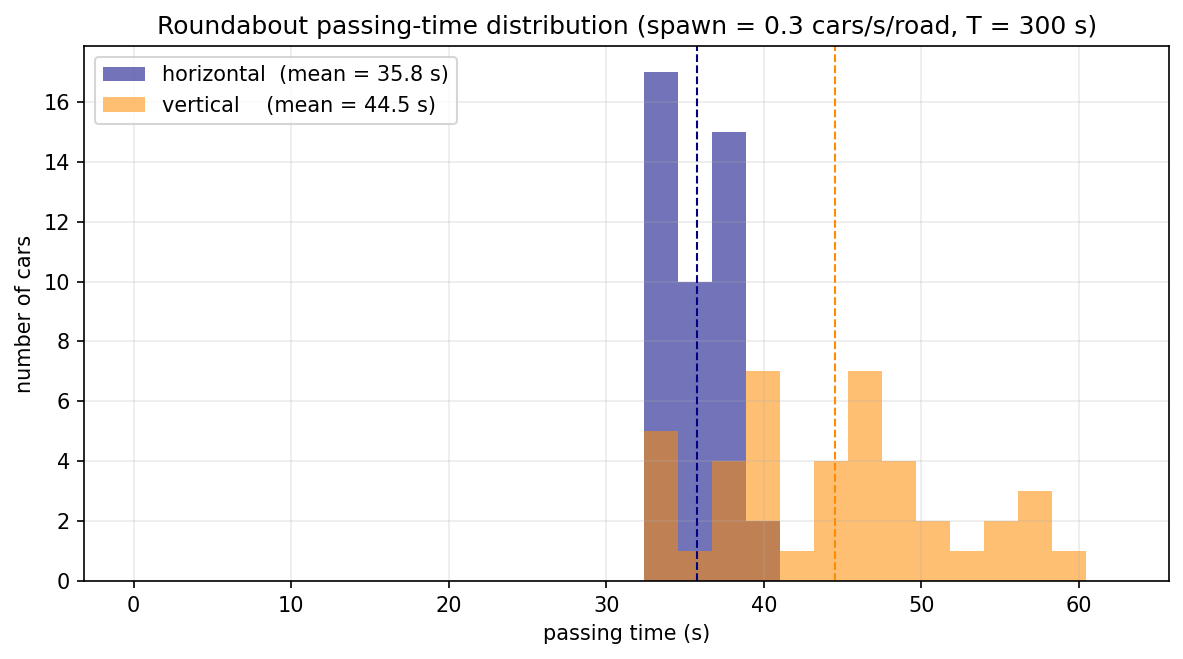
\includegraphics[width=0.85\textwidth]{fig_analysis1_roundabout_baseline.png}
    \caption{Baseline roundabout passing-time distribution at $r_H = r_V = 0.3$ cars/s. Horizontal cars cluster tightly near $36$ s; vertical cars sprawl out to $60$ s with mean $44.5$ s.}
\end{figure}

\end{document}
